\chapter{Assignment 3}
\section{Lecture 21.00 - Model 5, Example 1}
\begin{Example}{}{}
    A study of intoxication measured two groups of students,
    one of which was drunk while the other was not as
    they drove a computer-simulated driving course with a max speed limit of 50 km/h.
    Of interest was the maximum speed of an individual doing the computer-simulated driving
    course. Group 1 was intoxicated, while Group 2 was not.

    Is there a difference in speed between those that drive while
    intoxicated versus those that do not?

    \begin{itemize}
        \item \textbf{Data}:
              \begin{minted}{R}
# Data frames
grp1 <- c(50, 53, 52, 58)
grp2 <- c(62, 55, 58, 60)
# Must run to get same results as textbook
options(contrasts = c('contr.sum', 'contr.poly'))
Y <- c(grp1, grp2)
# Makes a discrete variable
x <- as.factor(c(rep(1, 4), rep(2, 4)))
# Builds the model
model <- lm(Y ~ x)
# Displays the output
summary(model)
        \end{minted}
        \item \textbf{Analysis}:
              \begin{minted}{R}
Call:
lm(formula = Y ~ x)

# (1)
Residuals:
   Min     1Q Median     3Q    Max 
 -3.75  -1.75  -0.50   1.75   4.75 

# (2), (4), (5)
Coefficients:
            Estimate Std. Error t value Pr(>|t|)    
(Intercept)   56.000      1.132  49.473 4.57e-09 ***
x1            -2.750      1.132  -2.429   0.0512 .  
---
Signif. codes:  0 ‘***’ 0.001 ‘**’ 0.01 ‘*’ 0.05 ‘.’ 0.1 ‘ ’ 1

# (3)
Residual standard error: 3.202 on 6 degrees of freedom
# Not important for this course.
Multiple R-squared:  0.4959,    Adjusted R-squared:  0.4119
# ANOVA, covered later in this course.
F-statistic: 5.902 on 1 and 6 DF,  p-value: 0.0512
\end{minted}
    \end{itemize}
    \begin{enumerate}[(1)]
        \item Helps test our residuals
        \item $ \hat{\mu}=56 $, $ \hat{\tau}_1=-2.75 $, $ \hat{\tau}_2=2.75 $
        \item $ \hat{\sigma}=3.202 $ on 6 degrees of freedom
        \item This line tests $ H_0 $: $ \mu=0 $ versus $ H_a $: $ \mu\ne 0 $
              \[ d=\frac{56-0}{1.132} =49.473 \]
              \[ p\text{-value}=2\Prob{D>49.473}=4.5\times 10^{-9} \]
              We have tons of evidence to reject $ H_0 $.
        \item $ H_0 $: $ \tau_1=0 $ versus $ H_a $: $ \tau_1\ne 0 $
              \[ d=\frac{-2.75-0}{1.132} =-2.429 \]
              \[ p\text{-value}=2\Prob{D>\abs{-2.429}}=2(1-\Prob{D\le 2.429})=0.0512 \]
              There is evidence to reject $ H_0 $.
    \end{enumerate}
    \underline{Questions}:
    \begin{itemize}
        \item \textbf{Q1}: What is the treatment effect for being inebriated?

              \textbf{Solution.} $ \hat{\tau}_1=-2.75 $ and $ \hat{\tau}_2=-\hat{\tau}_1=2.75 $
        \item \textbf{Q2}: Is there a difference between the treatment effect of group 1 and 2? Use a 95\% CI\@.

              \textbf{Solution.}
              \[ \theta=\text{ave of grp1}-\text{ave of grp2}=(\mu+\tau_1)-(\mu+\tau_2)=\tau_1-\tau_2 \]
              Estimator: $ \tilde{\theta}=\tilde{\tau}_1-\tilde{\tau}_2 $ and is normal by Gauss.
              \[ \E{\tilde{\theta}}=\E{\tilde{\tau}_1-\tilde{\tau}_2}=\E{\tilde{\tau}_1}-\E{\tilde{\tau}_2}=\tau_1-\tau_2 \]
              since unbiased.
              \[ \Var{\tilde{\theta}}
                  =\Var*{\bar{Y}_{1+}-\bar{Y}_{++}-(\bar{Y}_{2+}-\bar{Y}_{++})}
                  =\Var{\bar{Y}_{1+}-\bar{Y}_{2+}}
                  =\Var{\bar{Y}_{1+}}+\Var{\bar{Y}_{2+}}
                  =\frac{\sigma^2}{4} +\frac{\sigma^2}{4}
                  =\frac{\sigma^2}{2} \]
              CI for $ \theta $:
              \[ \theta:\hat{\theta}\pm c\,\text{SE}=\hat{\tau}_1-\hat{\tau}_2\pm
                  c\sqrt{\frac{\hat{\sigma}^2}{2}}\quad(c \sim t(n-q+c)=t(8-2+1)=t(6)) \]
              In our case,
              \[ \theta:(-2.75-2.75)\pm 2.447\sqrt{\frac{3.202^2}{2}}=(-11.04,0.04) \]
              $ 0 $ is in the interval, so we conclude that there is no difference
              between the treatment effect of group 1 and 2. In R, we could do
              \begin{minted}{R}
left <- -2.75 - 2.75 - qt(0.975, 6) * sqrt(summary(model)$sigma ^ 2 / 2)
right <- -2.75 - 2.75 + qt(0.975, 6) * sqrt(summary(model)$sigma ^ 2 / 2)
\end{minted}
              To obtain our CI $ \theta:(-11.039, 0.039) $.
        \item \textbf{Q3}: Is there a difference between the treatment effect of group 1 and 2? Use an HT\@.

              \textbf{Solution.} $ H_0 $: $ \tau_1=\tau_2 $ versus $ H_a $: $ \tau_1\ne \tau_2 $.
              \[ d=\frac{\hat{\tau}_1-\hat{\tau}_2-\tau_0}{\hat{\sigma}/\sqrt{2}}=
                  \frac{(-2.75-2.75)-0}{3.202/\sqrt{2}}=-2.489 \]
              \[ p=2\Prob{D\ge \abs{d}}=(0.05,0.10) \]
              We have some evidence to reject $ H_0 $. In R, we could do
              \begin{minted}{R}
d <- (-2.75 - 2.75) / (summary(model)$sigma / sqrt(2))
pval <- 2 * (1 - pt(abs(d), 6))
\end{minted}
              To obtain $ d=-2.429 $ and $ p\text{-value}=0.051 $. There is some difference
              between the treatment effect of group 1 and 2.
    \end{itemize}
\end{Example}
\section{Lecture 22.00 - Model 5, Example 1 Ctd}
We want to check our model assumpions of
$ R_j \sim \N{0,\sigma^2} $ independent. Four things to check:
\begin{itemize}
    \item $ \E{R_j}=0 $ (zero mean)
    \item $ \Var{R_j}=\sigma^2 $ (constant variance)
    \item Normality
    \item Independence
\end{itemize}
To check these, we can
\begin{itemize}
    \item plot residuals versus fitted values to check for both
          mean and variance assumption.

          \code{plot(model\$residuals)}
    \item qqplot to check for normality (straight line is normal).

          \code{qqnorm(model\$residuals)}
    \item residuals plot to check for independence assumption.

          \code{plot(model\$fitted.values, model\$residuals)}
\end{itemize}

\section{Lecture 23.00 - Model 5, Example 2}
\begin{Example}{}{m_5_ex_2}
    Suppose professors are coordinating 4 sections
    of the same course in a term. We want to look
    at the marks of each student for the midterm between these sections. The
    treatment is the ``instructor.''

    \begin{itemize}
        \item \textbf{Data}:
              \begin{minted}{R}
options(contrasts = c('contr.sum', 'contr.poly'))
Marks1 = c(55, 92, 48, 57, 66, 72)
Marks2 = c(62, 95, 84, 83, 66, 75)
Marks3 = c(89, 92, 94, 99, 87, 67)
Marks4 = c(25, 35, 71, 42, 44, 30)
Y = c(Marks1, Marks2, Marks3, Marks4)
\end{minted}
        \item \textbf{Analysis}:
              \begin{minted}{R}
x = as.factor(c(rep(1, 6), rep(2, 6), rep(3, 6), rep(4, 6)))
model = lm(Y ~ x)
summary(model)
\end{minted}

        \item \textbf{Output}:
              \begin{minted}{R}
Call:
lm(formula = Y ~ x)

Residuals:
     Min       1Q   Median       3Q      Max 
-21.0000 -10.2917   0.9167   6.1250  29.8333 

Coefficients:
            Estimate Std. Error t value Pr(>|t|)    
(Intercept)   67.917      2.861  23.741    4e-16 ***
x1            -2.917      4.955  -0.589 0.562699    
x2             9.583      4.955   1.934 0.067381 .  
x3            20.083      4.955   4.053 0.000621 ***
---
Signif. codes:  0 ‘***’ 0.001 ‘**’ 0.01 ‘*’ 0.05 ‘.’ 0.1 ‘ ’ 1

Residual standard error: 14.01 on 20 degrees of freedom
Multiple R-squared:  0.6506,    Adjusted R-squared:  0.5982 
F-statistic: 12.41 on 3 and 20 DF,  p-value: 8.281e-05
\end{minted}
    \end{itemize}


    Note that
    \begin{itemize}
        \item $ \hat{\tau}_4=-(\hat{\tau}_1+\hat{\tau}_2+\hat{\tau}_3)=-26.749 $
        \item $ \text{df}=n-q+c=(24)-(4+1)+1=20 $
    \end{itemize}
    \underline{Questions}:

    \textbf{Q1}: Is there a difference between the treatment effect of group 1 and 2? Use a 95\% CI\@.

    \textbf{Solution.} $ \tilde{\theta}=\tilde{\tau}_1+\tilde{\tau}_2 $ and by Gauss this
    is normal.
    \[ \E{\tilde{\theta}}=\E{\tilde{\tau}_1-\tilde{\tau}_2}=\tau_1+\tau_2 \]
    \[ \Var{\tilde{\theta}}=\Var{\tilde{\tau}_1-\tilde{\tau}_2}
        =\Var{\bar{Y}_{1+}-\bar{Y}_{2+}}
        =\Var{\bar{Y}_{1+}}+\Var{\bar{Y}_{2+}}
        =\frac{\sigma^2}{6} +\frac{\sigma^2}{6}
        =\frac{\sigma^2}{3} \]
    The 95\% confidence interval for $ \theta $ is
    \[ \hat{\tau}_1-\hat{\tau}_2 \pm c\, \frac{\hat{\sigma}}{\sqrt{3}}=
        -2.917-9.583\pm \frac{2.09(14.01)}{\sqrt{3}}=(-29.37,4.37) \quad(c \sim t(20))  \]
    In R, we could do
    \begin{minted}{R}
tau.1 <- summary(model)$coefficients[2]
tau.2 <- summary(model)$coefficients[3]
tau.3 <- summary(model)$coefficients[4]
tau.4 <- -1 * (tau.1 + tau.2 + tau.3)

tau.1 - tau.2 - qt(0.975, 20) * summary(model)$sigma/sqrt(3)
tau.1 - tau.2 + qt(0.975, 20) * summary(model)$sigma/sqrt(3)
\end{minted}
    To get at 95\% confidence interval $ \theta $: $ (-29.38,4.38) $. Yes,
    there is a difference between the treatment effect of group 1 and 2.

    \textbf{Q2}: Groups 2 and 3 were taught by the same instructor. Groups 1 and 4 are taught by another
    instructor. Is there a difference between the average treatment effect of instructor 1 to instructor 2? Use an
    HT\@.

    \textbf{Solution.}
    \[ \tilde{\theta}=\frac{\tilde{\tau}_1+\tilde{\tau}_4}{2}-\biggl(\frac{\tilde{\tau}_2+\tilde{\tau}_3}{2} \biggr)  \]
    \[ \E{\tilde{\theta}}=\frac{\tau_1+\tau_4}{2}-\biggl(\frac{\tau_2+\tau_3}{2} \biggr) \]
    \begin{align*}
        \Var{\tilde{\theta}}
         & =\Var*{\frac{\tilde{\tau}_1+\tilde{\tau}_4}{2}-\biggl(\frac{\tilde{\tau}_2+\tilde{\tau}_3}{2} \biggr) } \\
         & =\Var*{\frac{\bar{Y}_{1+}+\bar{Y}_{4+}}{2}-\biggl(\frac{\bar{Y}_{2+}+\bar{Y}_{3+}}{2} \biggr)}          \\
         & =\frac{1}{4} \Var{Y_{1+}}+\cdots+\frac{1}{4} \Var{Y_{4+}}                                               \\
         & =\frac{\sigma^2}{4(6)}+\cdots+\frac{\sigma^2}{4(6)}                                                     \\
         & =\frac{\sigma^2}{6}
    \end{align*}
    $ H_0 $: $ \theta=0 $ versus $ H_a $: $ \theta\ne 0 $.
    \[ d=\frac{\hat{\theta}-0}{\hat{\sigma}/\sqrt{6}}=-5.19\quad(D \sim t(20))  \]
    \[ p=2\Prob{D>\abs{-5.19}}=(0,0.001) \]
    We have tons of evidence to reject $ H_0 $. In R, we could do
    \begin{minted}{R}
theta <- ((tau.1 + tau.4) / 2) - ((tau.2 + tau.3) / 2)
d <- (theta - 0) / (summary(model)$sigma / sqrt(6))
pval <- 2 * (1 - pt(abs(d), 20))
\end{minted}
    To obtain a $ p $-value of $ 4.498007\times 10^{-5} $
\end{Example}
An example of a \emph{contrast} is
\[ \theta=\frac{\tau_1+\tau_4}{2} -\frac{(\tau_2+\tau_3)}{2}  \]
\begin{Definition}{Contrast}{}
    A \textbf{contrast} has the form
    \[ a_1\tau_1+a_2\tau_2+\cdots+a_n\tau_n \]
    where $ \sum_{i=1}^{n} a_i=0 $.
\end{Definition}

\section{Lecture 24.00 - ANOVA}
\underline{A}nalysis \underline{o}f \underline{V}ariance
\[ Y_{ij}=\mu+\tau_i+R_{ij}\quad(R_{ij}\sim \N{0,\sigma^2}) \]
Recall:
\begin{align*}
    W
     & =\sum_{ij}r_{ij}^2                                                      \\
     & =\sum_{ij}(y_{ij}-\hat{\mu}-\hat{\tau}_i)^2                             \\
     & =\sum_{ij}(y_{ij}-\hat{\mu})^2+(-r)\sum_{i}(\bar{y}_{i}-\bar{y}_{++})^2
\end{align*}
Rearranging
\[ \Uunderbracket{\sum_{ij}(y_{ij}-\bar{y}_{++})^2}_{\SS{Tot}}
    =\Uunderbracket{r \sum_{i}(y_{i+}-\bar{y}_{++})^2}_{\SS{Trt}}+
    \Uunderbracket{\sum_{ij}(y_{ij}-\hat{\mu}-\hat{\tau}_i)^2}_{\SS{Res}}   \]
\[ \boxed{\SS{Tot}=\SS{Trt}+\SS{Res}} \]
$ \SS{Tot} $
\begin{itemize}
    \item Represents a measure of \underline{total}
          variability in your data
    \item $ s^2=\dfrac{\SS{Tot}}{n-1}=\MS{Tot} $
    \item $ \text{df}=n-1 $
    \item You get this by fitting Model 1; $ Y_{i}=\mu+R_{i} $
          where $ R_i \sim \N{0,\sigma^2} $
    \item Recall $ \hat{\sigma}=s $ in Model 1
\end{itemize}
$ \SS{Res} $
\begin{itemize}
    \item The variability left over after you fit the model (unexplained)
    \item Synonymous with $ \hat{\sigma}^2 $
    \item $ \displaystyle \hat{\sigma}^2=\frac{W}{n-q+c} =\frac{\SS{res}}{\text{df}_{Res}}=\MS{Res} $
    \item $ \text{df}=n-q+c $
\end{itemize}
$ \SS{Trt} $
\begin{itemize}
    \item Due to $ \tau $ component
    \item $ \MS{Trt}=\dfrac{\SS{Trt}}{\text{df}_{\text{Trt}}} $
    \item $ \text{df}_{\text{Trt}}=t-1 $
    \item $ \boxed{\text{df}_{\text{Tot}}=\text{df}_{\text{Trt}}+\text{df}_{\text{Res}}} $
    \item Variability explained by your model
\end{itemize}
\[ \SS{Tot}=\SS{Trt}=\SS{Res} \]
We want $ \SS{Trt}\gg \SS{Res} $. We compare
$ \MS{Trt} $ to $ \MS{Res} $ using the ratio
\[ F=\frac{\MS{Trt}}{\MS{Res}} \]

\section{Lecture 25.00 - FTest}
\begin{figure}[!htbp]
    \centering
    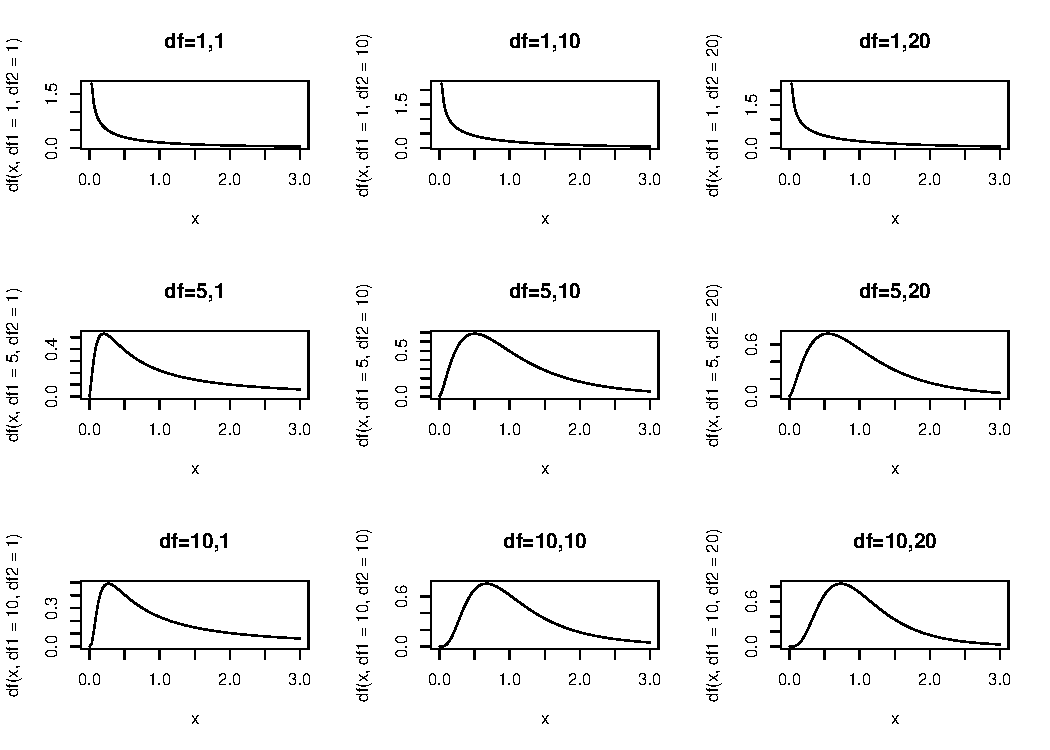
\includegraphics[width=0.7\textwidth]{fdistn.pdf}
    \caption{$ F $ distribution}
\end{figure}
\begin{Theorem}{}{}
    Let $ X \sim \chi^2(m) $ and $ Y \sim \chi^2(n) $, then
    \[ \frac{X/m}{Y/n} \sim F(m,n) \]
\end{Theorem}
\begin{Theorem}{}{}
    Let $ X \sim F(m,n) $ and $ Y \sim 1/X $, then
    \[ Y \sim F(n,m) \]
\end{Theorem}
\begin{Example}{}{}
    $ \alpha=\Prob{F(20,4)>4}=(0.05,0.1) $ since
    \begin{center}
        \begin{tabularx}{0.7\linewidth}{@{}YYYY@{}}
            $\alpha$       & 0.1  & 0.05 & 0.01 \\
            \midrule
            critical value & 3.84 & 5.80 & 14.0
        \end{tabularx}
    \end{center}
    In $ R $, we can directly calculate $ \alpha $ with \code{1-pf(4,20,4)=0.094}.
\end{Example}
\[ \tilde{F}=\frac{\tilde{\MS{Trt}}}{\tilde{\MS{Res}}}  \]
Now, $ \tilde{\MS{Res}}=\tilde{\sigma}^2 $. We know
\begin{equation}\label{eq:1}
    \frac{\tilde{\sigma}^2\text{df}_\text{Res}}{\sigma^2} \sim \chi^2(\text{df}_{\text{Res}})
\end{equation}
Similarly,
\begin{equation}\label{eq:2}
    \frac{\tilde{\MS{Trt}}\text{df}_\text{Trt}}{\sigma^2} \sim \chi^2(\text{df}_\text{Trt})
\end{equation}
Divide~\ref{eq:2} by~\ref{eq:1} to get
\[ \frac{\tilde{\MS{Trt}}}{\tilde{\MS{Res}}} \sim F(n,d) \]
where $ n=\text{df}_\text{Trt} $ and $ d=\text{df}_\text{Res} $.

\subsection*{When is $ F $ large?}
\[ \E{\tilde{F}}=
    \E*{\frac{\tilde{\MS{Trt}}}{\tilde{\MS{Res}}}}\approx
    \frac{\E{\tilde{\MS{Trt}}}}{\E{\tilde{\MS{Res}}}}
    =\frac{\sigma^2+r \dfrac{\sum_{i} \tau_i^2}{t-1} }{\sigma^2}  \]
\[ \E{\tilde{F}}=1+\frac{4}{\sigma^2} \frac{\sum \tau_i^2 }{t-1}  \]
If $ \tau_1=\tau_2=\cdots=\tau_t=0 $, then $ \E{\tilde{F}}=1 $.
However, if even one $ \tau $ is not zero, then $ \E{\tilde{F}}>1 $.

\subsection*{F Test}
\begin{enumerate}[(1)]
    \item $ H_0 $: $ \tau_1=\tau_2=\cdots=\tau_t=0 $ versus $ H_a $: at least one $\tau$ is not zero.
    \item $ \displaystyle d=\frac{\MS{Trt}}{\MS{Res}}  $ where $ D \sim F(\text{df}_\text{Trt},\text{df}_\text{Res}) $
    \item $ p\text{-value}=\Prob{D>d} $
    \item Conclusion.
\end{enumerate}

\section{Lecture 26.00 - FTest, Example}
\begin{Example}{F Test}{}
    See~\Cref{ex:m_5_ex_2} for the data.
    \begin{minted}{R}
anova(model)
Analysis of Variance Table

Response: Y
          Df Sum Sq Mean Sq F value    Pr(>F)    
x          3 7315.5 2438.50  12.415 8.281e-05 ***
Residuals 20 3928.3  196.42                      
---
Signif. codes:  0 ‘***’ 0.001 ‘**’ 0.01 ‘*’ 0.05 ‘.’ 0.1 ‘ ’ 1
    \end{minted}
    \begin{itemize}
        \item $ H_0 $: $ \tau_1=\tau_2=\tau_3=\tau_4=0 $
        \item $ H_a $: At least one $ \tau $ is not zero
    \end{itemize}
    \[ d=\frac{\MS{Trt}}{\MS{Res}} =\frac{\SS{Trt}/\text{df}_\text{Trt}}{\SS{Res}/\text{df}_\text{Res}}
        =\frac{7315.5/3}{3928.3/20}=12.415   \]
    Note that $ D \sim F(3,20) $, so
    \[ p=\Prob{D>12.415}=8.21 \times 10^{-5} \]
    We have tons of evidence against $ H_0 $.
\end{Example}
